% flashcards-title: A mixed collection of triangles and circles
% flashcards-desc: Two rows of small shapes arranged in mixed order. Some of the shapes are gold triangles and the others are pale circles with dark outlines.
\documentclass[tikz]{standalone}
\usetikzlibrary{arrows.meta,patterns}

\definecolor{qraNavy}{HTML}{17324D}
\definecolor{qraBlue}{HTML}{2B6CB0}
\definecolor{qraGold}{HTML}{B7791F}
\definecolor{qraPale}{HTML}{EAF2F8}
\definecolor{qraGray}{HTML}{5C6773}

\tikzset{
  qra axis/.style={draw=qraNavy, line width=1.2pt},
  qra tick/.style={draw=qraNavy, line width=1pt},
  qra guide/.style={draw=qraGray, densely dashed, line width=0.8pt},
  qra counter/.style={circle, draw=qraNavy, fill=qraPale, line width=0.9pt, minimum size=7mm, inner sep=0pt},
  qra label/.style={font=\sffamily\bfseries, text=qraNavy},
  qra small label/.style={font=\sffamily, text=qraNavy},
}

\begin{document}
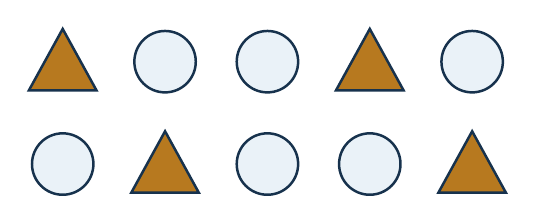
\begin{tikzpicture}[x=1.3cm, y=1.3cm]
  % Row layout (top then bottom): T C C T C / C T C C T
  % 4 triangles and 6 circles in all.
  \newcommand{\shapecircle}[2]{\draw[qraNavy, line width=0.9pt, fill=qraPale] (#1,#2) circle (0.30);}
  \newcommand{\shapetriangle}[2]{\draw[qraNavy, line width=0.9pt, fill=qraGold] (#1-0.33,#2-0.28) -- (#1+0.33,#2-0.28) -- (#1,#2+0.32) -- cycle;}
  % Top row
  \shapetriangle{0}{1}
  \shapecircle{1}{1}
  \shapecircle{2}{1}
  \shapetriangle{3}{1}
  \shapecircle{4}{1}
  % Bottom row
  \shapecircle{0}{0}
  \shapetriangle{1}{0}
  \shapecircle{2}{0}
  \shapecircle{3}{0}
  \shapetriangle{4}{0}
\end{tikzpicture}
\end{document}
